\chapter{Prototipos estructurales}\label{cap:prototipos}

% --- INTRODUCCIÓN  ---

El análisis independiente de precipitación total (Capítulo~\ref{cap:resultados_tp}) y viento a 10 metros (Capítulo~\ref{cap:resultados_wind10}) muestra que ambas variables experimentan transformaciones estructurales profundas y distintas a lo largo del ciclo de vida ciclónico, en función de la intensidad dinámica del sistema. Sin embargo, el análisis separado no permite cuantificar la diferenciación espacial conjunta entre circulación y precipitación en un mismo marco de referencia. Para cerrar esta brecha, este capítulo introduce el \textit{prototipo estructural acoplado}, una visualización que superpone, en el mismo dominio centrado en el sistema, los campos de densidad de probabilidad espacial (PDFe) y los patrones EOF dominantes de ambas variables.

Cada prototipo combina cuatro capas de información geométrica: (i) los contornos PDFe de los cuantiles 75 y 90 para precipitación (azul) y viento (rojo), que mapean las zonas de mayor concentración probabilística de máximos; (ii) las cargas positiva (sólida) y negativa (punteada) del primer modo EOF de ambas variables (verde para precipitación, naranja para viento); y (iii) las coordenadas modales ($\Delta x$, $\Delta y$) de cada campo respecto al centro del vórtice (0,0), representadas mediante estrellas. El dominio de análisis corresponde al marco de $20^{\circ} \times 20^{\circ}$ centrado en el núcleo ciclónico, delimitado por una máscara circular de radio $9{,}5^{\circ}$. Se presentan dos versiones: la Población Global (Fig.~\ref{fig:prototipo_global}) y el subconjunto de ciclones de alta vorticidad p90 (Fig.~\ref{fig:prototipo_p90}), organizadas en una matriz de $3 \times 4$ paneles (regiones $\times$ fases evolutivas).

Esta construcción usa los patrones EOF1 univariados de cada campo (Capítulos~\ref{cap:resultados_wind10} y \ref{cap:resultados_tp}), calculados de forma independiente, en vez del modo conjunto MEOF1 (Capítulo~\ref{chap:meof}). La razón es que, en varias combinaciones de región, fase y población, el MEOF1 está dominado casi por completo por el viento (Sección~\ref{sec:discusion_meof}), por lo que la carga de precipitación dentro de ese modo conjunto no siempre refleja la variabilidad propia de la precipitación. Cada EOF1 univariado, en cambio, cuenta con su propia prueba de significancia y varianza explicada, verificadas por separado en los capítulos correspondientes. La contrapartida de esta elección es que la separación geométrica entre los centros modales de viento y precipitación combina dos descomposiciones independientes, por lo que no está garantizada por construcción, sino respaldada de forma indirecta por la correlación negativa y significativa entre sus componentes principales en madurez p90 (Sección~\ref{sec:meof_coherencia}). En esa misma combinación, el MEOF1 también muestra una contribución comparable de ambos campos (Capítulo~\ref{chap:meof}, Tabla~\ref{tab:meof_bias_check}), por lo que la geometría resultante no depende de forma crítica de cuál de las dos descomposiciones se use.

\section{Población Global}\label{sec:prototipo_global}

\begin{figure}[H]
\centering
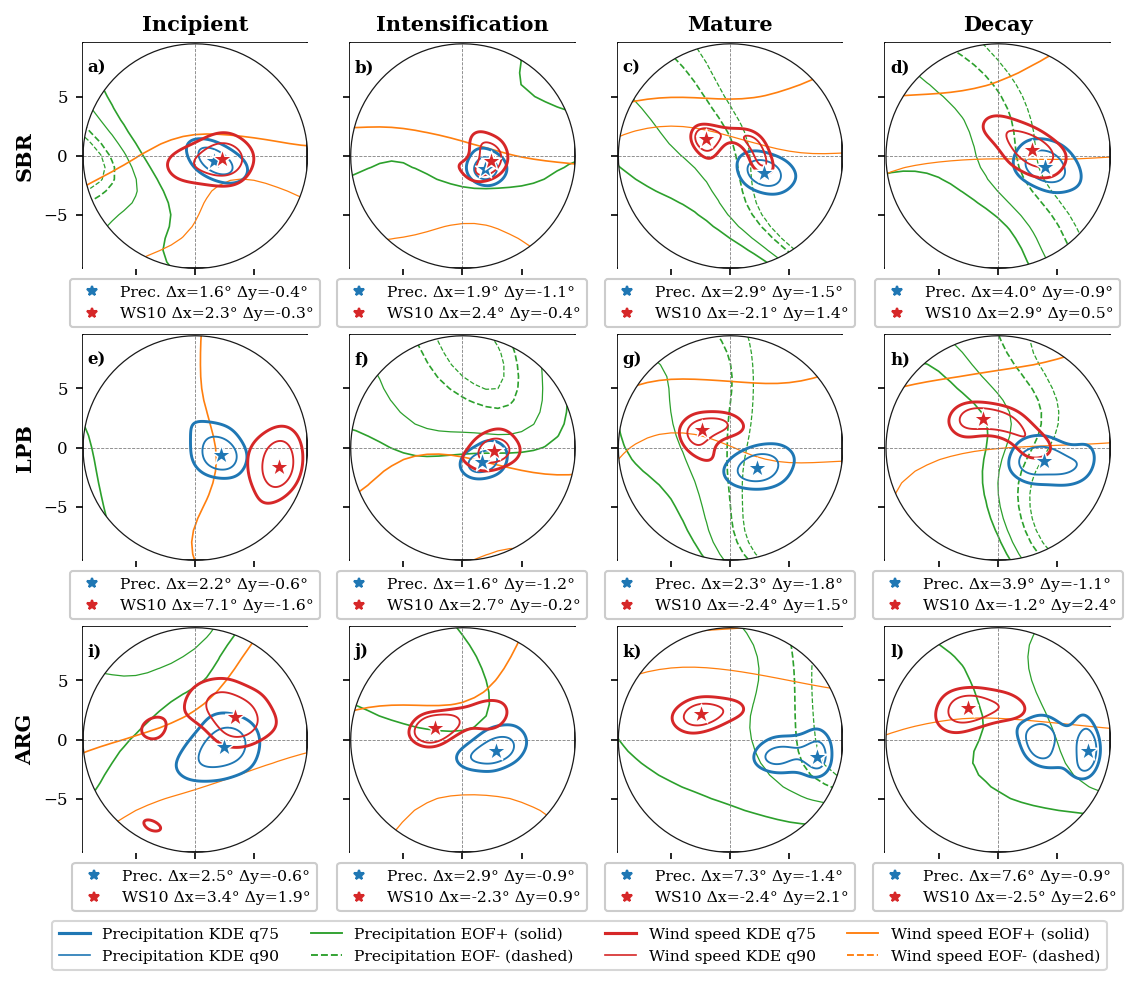
\includegraphics[width=\textwidth]{images/prototipos/prototipo_12panels_global.png}
\caption[Prototipos estructurales acoplados — Población Global]{Prototipos estructurales acoplados para la Población Global de ciclones extratropicales del Atlántico Sudoccidental. Cada panel superpone en el dominio de $20^{\circ} \times 20^{\circ}$ centrado en el sistema (0,0) los contornos PDFe de los cuantiles 75 y 90 de precipitación total (azul, línea gruesa y delgada respectivamente) y viento a 10 m (rojo), junto con las cargas positivas (línea sólida) y negativas (línea punteada) del EOF1 de precipitación (verde) y viento (naranja). Las estrellas azul y roja indican las coordenadas modales ($\Delta x$, $\Delta y$) de cada campo. La matriz organiza las regiones de ciclogénesis en filas (SBR, LPB, ARG) y las fases evolutivas en columnas (Incipiente, Intensificación, Madurez, Decaimiento). La máscara circular delimita el dominio a un radio de $9{,}5^{\circ}$.}
\label{fig:prototipo_global}
\end{figure}

La Figura~\ref{fig:prototipo_global} presenta los prototipos estructurales acoplados para la Población Global, integrando la geometría probabilística de los máximos de ambas variables con los patrones de mayor variabilidad explicada (EOF1) para ofrecer una lectura simultánea de la ubicación preferencial de los forzantes de precipitación y circulación a lo largo del ciclo de vida.

Se construye a partir de los campos PDFe sobre la grilla fija centrada en el sistema (Sección~\ref{subsec:kde_tp_global} para precipitación y Sección~\ref{sec:kde_espacial_global} para viento), combinados con el primer autovector espacial de los análisis EOF independientes (Sección~\ref{sec:eof_tp} y Sección~\ref{sec:eof_wind10}). Los contornos de densidad se suavizan con un filtro gaussiano ($\sigma = 2$) antes de trazar los niveles de los cuantiles 75 y 90 según el criterio de región de mayor densidad (HDR). Su propósito es sintetizar la coexistencia o diferenciación espacial entre circulación y precipitación en los ciclones ordinarios, estableciendo la línea base frente a la cual se comparará el subconjunto de alta vorticidad en la sección siguiente.

Durante las fases incipiente e intensificación (paneles a--f), los prototipos de la Población Global muestran una co-localización relativa entre los máximos de precipitación y viento. En SBR (paneles a--b), los contornos PDFe se superponen parcialmente en el cuadrante oriental, con las modas de precipitación y viento separadas apenas $0{,}1^{\circ}$--$0{,}7^{\circ}$ en latitud, mientras las cargas del EOF1 de viento se extienden hacia el noroeste. En LPB (paneles e--f), tanto la precipitación como el viento se sitúan al este-sureste del centro durante la incipiencia, con el viento sistemáticamente más alejado en la componente zonal. La separación modal es de $4{,}9^{\circ}$ en la fase incipiente (panel e) y se reduce a $1{,}1^{\circ}$ en la intensificación (panel f). En ARG (paneles i--j), el patrón ya es bimodal desde las etapas tempranas. El PDFe de precipitación se mantiene al este-sureste en ambas fases, mientras el de viento se desplaza del noreste (panel i) al noroeste (panel j), anticipando la divergencia que se consolida en la madurez. Esta co-localización parcial inicial refleja que, en el régimen promedio, los forzantes frontales del WCB organizan ambos campos en el mismo sector activo del ciclón, antes de que la diferenciación interna imponga geometrías distintas.

Al transitar hacia la madurez (paneles c, g, k) y el decaimiento (paneles d, h, l), la arquitectura del prototipo se modifica de forma sistemática aunque moderada. En LPB, los contornos PDFe de viento se desplazan hacia el noroeste, coherentemente con la intensificación de la circulación en el flanco posterior del ciclón, mientras los de precipitación se expanden hacia el este y sureste, alcanzando una separación zonal de $4{,}7^{\circ}$ en la madurez (panel g) que se mantiene en $5{,}1^{\circ}$ en el decaimiento (panel h). En SBR este patrón es menos consistente. La separación zonal de $5{,}0^{\circ}$ observada en la madurez (panel c) se reduce a $1{,}1^{\circ}$ en el decaimiento (panel d), donde el viento retorna hacia el sector nororiental en lugar de continuar desplazándose al occidente. Sin embargo, tanto los contornos PDFe como las cargas EOF1 mantienen en la Población Global una extensión espacial considerable, sin que ningún campo colapse hacia una geometría angosta y bien definida, comportamiento que refleja la heterogeneidad estructural inherente al catálogo completo, donde la integración de ciclones con distintas tasas de oclusión, profundidades de vórtice y ambientes termodinámicos diluye la señal espacial de cualquier subconjunto estructuralmente coherente.

La comparación regional revela asimetrías en la dinámica de separación. En ARG (paneles i--l), la divergencia entre los PDFe de viento y precipitación es la más pronunciada desde las fases iniciales, con la moda de viento desplazada hacia el noroeste ($\Delta x < 0$, $\Delta y > 0$) a partir de la intensificación (paneles j--l), tras iniciar al noreste en la fase incipiente (panel i, $\Delta x = 3{,}4^{\circ}$, $\Delta y = 1{,}9^{\circ}$), mientras la moda de precipitación se mantiene al este-sureste, con $\Delta x$ positivo y $\Delta y$ negativo en los cuatro paneles. Este comportamiento contrasta con SBR y LPB, donde la separación meridional es menor y la distribución de precipitación es más extensa, reflejando el mayor acceso a humedad oceánica y la mayor variabilidad de trayectorias de las celdas de precipitación. Estas diferencias regionales son coherentes con los patrones individuales descritos en los capítulos anteriores y confirman que la síntesis estructural del prototipo no promedia estas diferencias sino que las preserva en la lectura integrada.

\section{Subconjunto de alta vorticidad (p90)}\label{sec:prototipo_p90}

\begin{figure}[H]
\centering
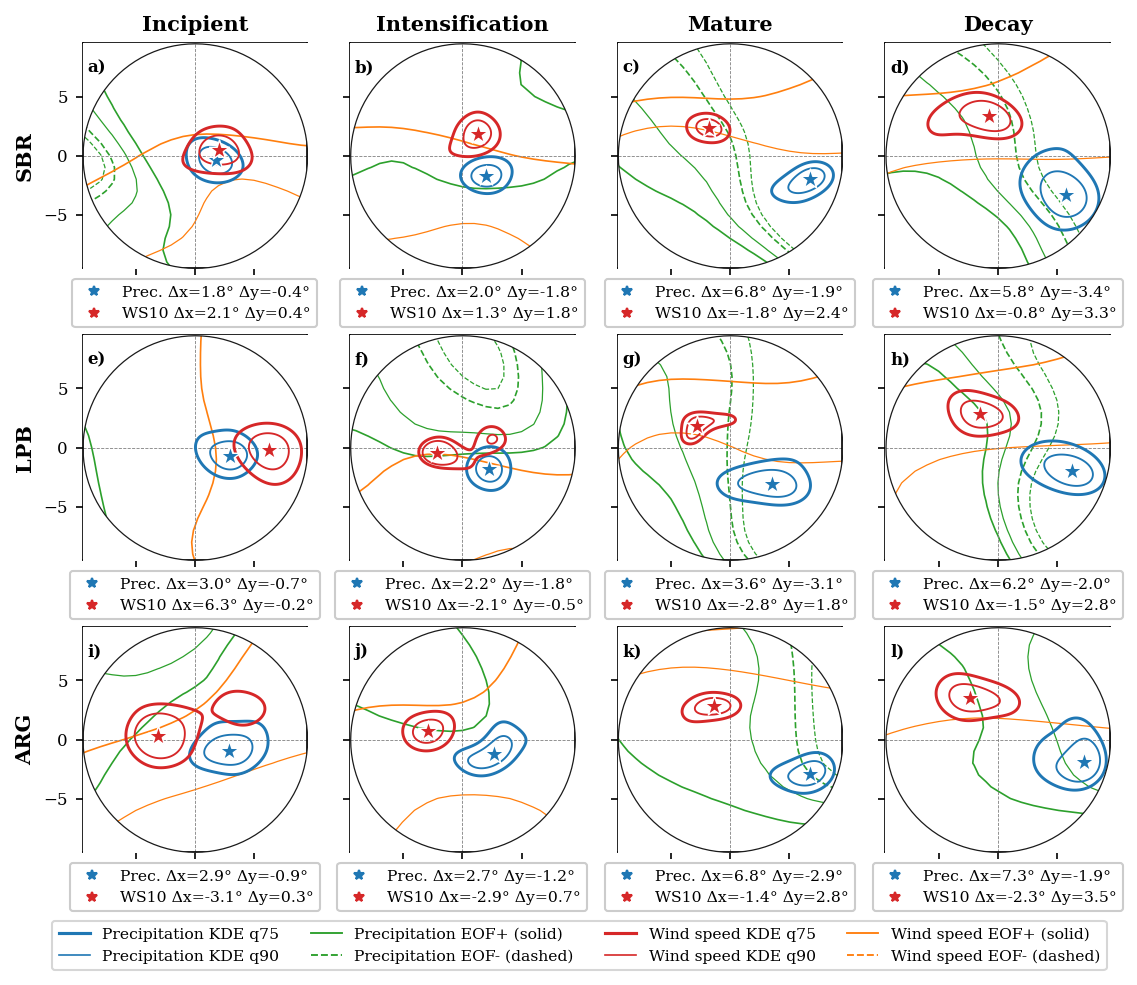
\includegraphics[width=\textwidth]{images/prototipos/prototipo_12panels_p90.png}
\caption[Prototipos estructurales acoplados — Subconjunto p90]{Prototipos estructurales acoplados para el subconjunto de ciclones de alta vorticidad (percentil 90 de vorticidad máxima). El formato de paneles, la disposición matricial ($3 \times 4$, regiones $\times$ fases), la simbología de colores y la escala del dominio centrado en el sistema son idénticos a los de la Figura~\ref{fig:prototipo_global}, permitiendo cuantificar directamente la transformación estructural que experimentan los sistemas p90 respecto a la climatología general.}
\label{fig:prototipo_p90}
\end{figure}

La Figura~\ref{fig:prototipo_p90} presenta los prototipos estructurales acoplados para el subconjunto de ciclones de alta vorticidad (p90), construidos con el mismo procedimiento metodológico que la Figura~\ref{fig:prototipo_global} pero restringidos al estrato de sistemas con vorticidad máxima en el percentil 90. Esta visualización cuantifica la diferenciación espacial entre circulación y precipitación en los sistemas p90 del Atlántico Sudoccidental, cerrando el argumento analítico desarrollado en los capítulos de precipitación y viento. La comparación directa entre ambas figuras, posible gracias a la escala, simbología y disposición matricial idénticas, permite evaluar si la intensificación dinámica amplifica o reorganiza la arquitectura de acoplamiento entre variables.

El contraste visual con la Población Global es inmediato y profundo. En la fase de madurez de SBR (panel c), el PDFe de precipitación (azul) colapsa hacia una estructura compacta desplazada hacia el este-sureste ($\Delta x = 6{,}8^{\circ}$, $\Delta y = -1{,}9^{\circ}$), mientras el PDFe de viento (rojo) se concentra en el cuadrante noroeste ($\Delta x = -1{,}8^{\circ}$, $\Delta y = 2{,}4^{\circ}$). La separación angular entre ambas modas supera los $8^{\circ}$ en distancia euclídea, en contraste con los ${\sim}5{,}8^{\circ}$ observados en el mismo panel (SBR, madurez) de la Población Global. Esta brecha no es uniforme entre regiones y fases en la Población Global: en SBR, la separación en las fases tempranas es mínima (paneles a-b, $0{,}7^{\circ}$--$0{,}9^{\circ}$), pero en LPB y ARG ya se observan separaciones considerables incluso en incipiencia e intensificación (hasta $5{,}5^{\circ}$ en la intensificación de ARG, panel j), de modo que el contraste Global-vs-p90 es más marcado en SBR que en las otras dos regiones. Este patrón de separación cruzada, precipitación al este-sureste, viento al noroeste, se reproduce con notoria consistencia en LPB (paneles g y h) y, con la mayor magnitud de las tres regiones, en ARG (paneles k y l), donde la precipitación se desplaza hacia el este ($\Delta x = 6{,}8^{\circ}$) y el viento mantiene su posición al noroeste ($\Delta x = -1{,}4^{\circ}$, $\Delta y = 2{,}8^{\circ}$), alcanzando una separación euclídea cercana a $10^{\circ}$ en la madurez, que se amplía aún más en el decaimiento (panel l, ${\sim}11^{\circ}$), la mayor de todo el subconjunto p90. Esta firma geométrica de cuadrantes opuestos constituye la expresión cuantitativa de la diferenciación espacial entre campos en los ciclones p90 de la región.

La génesis de esta diferenciación en los sistemas de alta vorticidad podría estar relacionada con los procesos de oclusión documentados en los análisis individuales de cada variable: la alta concentración del viento en el cuadrante noroeste, con densidades de hasta 27$\times10^{-4}$ en SBR y 23--25$\times10^{-4}$ en LPB (ARG se mantiene más baja, ${\sim}19$--$21\times10^{-4}$; Sección~\ref{sec:kde_espacial_p90}), y la concentración del EOF1 de precipitación de hasta 36.5\% en LPB durante el decaimiento (Sección~\ref{subsec:var_exp_tp}), son las dos caras cuantitativas de la misma reorganización que aquí se sintetiza. El patrón de viento al noroeste es compatible con el ciclo de vida tipo Shapiro-Keyser \citep{shapiro1990life}, en el que la cinta transportadora fría (\textit{cold conveyor belt}, CCB) se enrollaría alrededor del núcleo del sistema en proceso de oclusión, generando el máximo de circulación de bajo nivel en el sector posterior del vórtice \citep{schemm2014linkage}. Simultáneamente, una posible intrusión seca (\textit{dry intrusion}) desde la alta troposfera hacia el núcleo del ciclón explicaría el espacio relativamente libre de precipitación que separa ambos campos, aunque este mecanismo no se mide directamente en ningún capítulo de esta tesis. El remanente de humedad del WCB, por su parte, es arrastrado por la circulación ciclónica hacia la periferia, formando la estructura en arco de precipitación en el cuadrante este-sureste, en una posición más cercana a la del WCB que a la del cuadrante ocluido que \citet{martin1999forcing} describe para la banda enroscada (\textit{wrap-around precipitation}). La superposición de estos dos procesos, operando en cuadrantes opuestos, es lo que genera la configuración diferenciada que captura el prototipo p90.

La fase de decaimiento (paneles d, h, l) consolida y exacerba esta separación en los tres regímenes regionales. En SBR (panel d), la moda de precipitación se desplaza aún más hacia el sur ($\Delta x = 5{,}8^{\circ}$, $\Delta y = -3{,}4^{\circ}$) mientras el viento migra al norte ($\Delta x = -0{,}8^{\circ}$, $\Delta y = 3{,}3^{\circ}$), aumentando la separación euclídea a más de $9^{\circ}$. En LPB (panel h), los contornos PDFe de precipitación se estrechan en una banda arqueada hacia el sur-sureste, en tanto el viento mantiene su núcleo compacto al noroeste, con una separación modal de $7{,}7^{\circ}$ en la dirección zonal. Este comportamiento refleja que, a medida que el ciclón se disipa, la estructura en arco mantiene su posición periférica incluso cuando la intensidad del sistema se debilita, mientras que el núcleo de viento se sostiene por la inercia ciclónica y la advección de vorticidad remanente. Las cargas del EOF1 de viento (naranja) mantienen su orientación noroeste-suroeste en todas las regiones durante el decaimiento, mientras que las del EOF1 de precipitación (verde) adquieren una curvatura arqueada hacia el sur, coherente con la geometría de la banda periférica documentada en la Sección~\ref{subsec:eof1_tp_p90}.

Las diferencias regionales en la geometría de la separación se manifiestan primero en la intensidad y extensión del campo de precipitación. En SBR y LPB, la disponibilidad de humedad tropical canalizada por el SALLJ \citep{reboita2026meteorology} podría sostener la estructura en arco de precipitación con mayor intensidad, incrementando la densidad en el cuadrante sureste y ensanchando la zona de alta probabilidad en la madurez y el decaimiento. En ARG (paneles i--l), la correlación entre el PC1 de precipitación y la vorticidad se mantiene significativa durante todo el ciclo de vida en p90, incluida la madurez (Capítulo~\ref{cap:resultados_tp}), a diferencia de SBR y LPB, donde esa correlación deja de ser significativa en esta fase, lo que podría explicar que la banda de precipitación, aunque más difusa en términos de densidad PDFe, mantenga una posición consistente; sin embargo, la separación euclídea entre las modas de viento y precipitación no resulta menor que en SBR y LPB, sino la mayor de las tres regiones (${\sim}10$--$11^{\circ}$ en madurez y decaimiento, frente a ${\sim}9$--$9{,}5^{\circ}$ en SBR y ${\sim}8$--$9^{\circ}$ en LPB). La dirección de la diferenciación, precipitación al este-sureste, viento al noroeste, sí se mantiene consistente en las tres regiones, revelando que la topología fundamental de la reorganización espacial es común a las tres regiones, mientras que su magnitud responde a una combinación de factores regionales que este capítulo no logra atribuir de forma unívoca al régimen de humedad oceánica.

La fase incipiente de los ciclones de alta vorticidad (paneles a, e, i) muestra que la diferenciación aún no está plenamente desarrollada, pero ya exhibe una tendencia diferenciada respecto a la Población Global equivalente. En SBR (panel a), la moda de viento al noreste ($\Delta x = 2{,}1^{\circ}$, $\Delta y = 0{,}4^{\circ}$) se separa levemente de la moda de precipitación al este ($\Delta x = 1{,}8^{\circ}$, $\Delta y = -0{,}4^{\circ}$), con los contornos PDFe aún parcialmente superpuestos pero con centros diferenciados; la orientación hacia el noroeste que caracterizará al viento en fases posteriores todavía no se manifiesta en esta etapa incipiente. En LPB (panel e), la separación zonal es más notable desde el inicio ($\Delta x_{\text{viento}} = 6{,}3^{\circ}$, $\Delta x_{\text{prec}} = 3{,}0^{\circ}$), reflejando que los sistemas que eventualmente alcanzarán el percentil 90 de vorticidad ya exhiben durante su génesis una asimetría frontal más pronunciada que el promedio, coherente con el mayor gradiente térmico y el mayor flujo de humedad que caracteriza a estos entornos de ciclogénesis más activos.

% SECCIÓN: DISCUSIÓN
\section{Discusión}\label{sec:discusion_prototipos}

% --- PÁRRAFO 1: Validación del enfoque centrado en el sistema y comparación con literatura ---

La co-localización parcial documentada en los prototipos de la Población Global durante las fases incipiente e intensificación --consistente con el pico modal simultáneo de viento (12--15~m\,s$^{-1}$) y precipitación (10--20~mm/h) ya reportado en esa misma fase (Secciones~\ref{sec:pdf_wind10} y~\ref{sec:pdf_tp})-- es coherente con los resultados de \citet{cardoso2022synoptic} para ciclones subtropicales del Atlántico Sur, una estructura generalmente distinta de los ETC baroclínicos catalogados en esta tesis, quienes, mediante un marco lagrangiano similar, con un dominio de $20^{\circ} \times 20^{\circ}$ que sigue al centro del ciclón, identifican anomalías positivas de viento al este y noreste de la región ciclogenética RG1 y de precipitación al este y dentro de ella, promediadas sobre el ciclo de vida. Los prototipos del presente trabajo extienden este resultado de dos maneras: primero, al incorporar explícitamente la fase evolutiva como eje de estratificación, muestran que esta co-localización es propia de las fases tempranas y no una propiedad estática del ciclón; segundo, al contrastar la Población Global con el subconjunto p90, muestran que la co-localización se quiebra de manera cuantificable en los sistemas p90. Esta distinción no puede inferirse de los análisis climatológicos que promedian el ciclo de vida completo \citep{gramcianinov2023impact}, y constituye el valor agregado central del enfoque de prototipos condicionales adoptado en esta tesis.

% --- PÁRRAFO 2: El desacople espacial en p90 y el modelo Shapiro-Keyser ---

La separación de cuadrantes en los prototipos p90, viento al noroeste, precipitación al sureste y sur, es compatible con la transición al modelo de Shapiro-Keyser \citep{shapiro1990life}. Esta interpretación se apoya en un modelo conceptual general, sin un estudio equivalente para el Atlántico Sur que confirme directamente la secuencia completa de oclusión en esta región.

% --- PÁRRAFO 3: Comparación con estudios del Hemisferio Norte y transferibilidad del marco conceptual ---

La arquitectura de cuadrantes documentada en los prototipos p90 del Hemisferio Sur guarda cierta correspondencia, aunque especular, con la organización del campo de viento reportada para ciclones explosivos del Hemisferio Norte. \citet{priestley2022improved} componen los sistemas del percentil 90 de vorticidad ciclónica en ERA5 sobre un dominio de ${\sim}20^{\circ}$ centrado en la trayectoria, criterio y escala comparables a los de este trabajo, y encuentran que los vientos asociados a la CCB se concentran en el flanco posterior-occidental del vórtice; por inversión de la circulación ciclónica entre hemisferios, esta posición es topológicamente análoga a la concentración noroeste del viento documentada aquí. Cabe precisar que dicho estudio no analiza el campo de precipitación, por lo que la comparación se limita estrictamente al viento.

Las diferencias observadas, particularmente la mayor difusión de los contornos en el sector sur y la asimetría meridional más pronunciada en SBR, son consistentes con la mayor disponibilidad de humedad subtropical en la región. \citet{gozzo2014subtropical} documentan ciclones subtropicales en el Atlántico Sur, una categoría distinta de los ETC catalogados en esta tesis, por lo que la posible estructura híbrida de los sistemas p90 no se verifica aquí. Esto sugiere que la organización del viento en cuadrantes opuestos al forzante del WCB es un rasgo compartido entre hemisferios, mientras que la geometría de la estructura en arco de precipitación del Atlántico Sur no tiene un análogo conjunto viento-precipitación documentado en la literatura del Hemisferio Norte consultada aquí.

% --- PÁRRAFO 4: Los prototipos como herramienta de diagnóstico: vínculo con el marco multivariado ---

El enfoque de prototipos estructurales desarrollado en este capítulo se alinea metodológicamente con propuestas recientes que enfatizan la necesidad de vincular explícitamente la evolución dinámica del sistema con sus manifestaciones estructurales. \citet{han2025system} proponen \textit{SyCLoPS}, un marco de clasificación objetiva de alcance global que distingue dieciséis clases de sistemas de baja presión, incluidos los ciclones extratropicales como la clase más frecuente de su catálogo. Sin embargo, su marco reserva la designación de sistemas de \textit{alto impacto}, y los composites de estructura, precipitación y energía cinética asociados a esa designación, a los ciclones tropicales, subtropicales y bajas polares, sin incluir a los ciclones extratropicales en ese análisis pese a ser la clase más frecuente de su catálogo. Los prototipos presentados en este capítulo abordan ese vacío para el Atlántico Sur, cuantificando mediante densidades de probabilidad espacial y modos dominantes de variabilidad (EOF) la posición relativa de los máximos de viento y precipitación respecto al centro del vórtice, en un dominio centrado en el sistema estandarizado que permite la comparación directa entre regiones y fases del ciclo de vida. Esta aproximación revela, para los ciclones extratropicales de la región, una reorganización geométrica horizontal entre ambos campos que un composite de corte vertical no captura directamente. Esta combinación de geometría modal y densidad probabilística constituye, al igual que el marco propuesto por \citet{corner2025classification} mediante análisis multivariado de parámetros dinámicos, un avance hacia la caracterización objetiva y cuantificada de los sistemas intensos ($\zeta_{850}$) en el Atlántico Sur, una región donde estudios equivalentes han permanecido hasta ahora muy limitados.

% --- PÁRRAFO 5: Limitaciones del enfoque y perspectivas futuras ---

Dos limitaciones del enfoque de prototipos merecen discusión explícita. En primer lugar, la estandarización del dominio centrado en el sistema en una grilla fija de $\pm 9{,}5^{\circ}$ implica que sistemas cuya estructura en arco de precipitación se extiende más allá de este radio, posible en los ciclones de mayor escala horizontal, contribuyen con densidad PDFe truncada en los bordes del dominio, subestimando la extensión real del campo de precipitación en el prototipo. Esta limitación es inherente al enfoque composito centrado y ha sido reconocida por \citet{cardoso2022synoptic}, quienes adoptan explícitamente un dominio de $20^{\circ} \times 20^{\circ}$ precisamente para capturar los vientos extremos que pueden ocurrir hasta 500 km del centro del ciclón. En segundo lugar, la construcción de los prototipos sobre el subconjunto estático p90 de vorticidad máxima implica que la muestra incluye sistemas en distintas fases de su ciclo de vida al momento de ser catalogados, aunque la estratificación por fases mediante el algoritmo \textit{CycloPhaser} \citep{deSouza2025CycloPhaser} mitiga en gran medida este efecto al garantizar que cada instante analizado pertenece a la fase correcta del ciclón individual. Estas limitaciones abren líneas de trabajo futuro: la extensión del dominio a $30^{\circ} \times 30^{\circ}$ para ciclones de gran escala, y la estratificación adicional por velocidad de traslación del sistema, un factor que, como señalan \citet{gramcianinov2023impact}, modula directamente la duración del forzante y la extensión espacial de los campos dinámicos, permitirían refinar los prototipos hacia representaciones más completas de la diversidad estructural de los ciclones de alta vorticidad del Atlántico Sur.

\section{Síntesis}\label{sec:sintesis_prototipos}

Los prototipos estructurales acoplados sintetizan, en una representación geométrica única, la evolución diferencial de la organización espacial de los campos de precipitación y viento asociada a los ciclones extratropicales del Atlántico Sudoccidental a lo largo de su ciclo de vida. En la Población Global, los campos de precipitación y viento exhiben durante las fases incipiente e intensificación una co-localización relativa en el cuadrante oriental, con separaciones modales moderadas que reflejan la organización frontal del WCB como forzante común. A medida que los sistemas evolucionan hacia la madurez y el decaimiento, los campos se separan gradualmente manteniendo geometrías difusas que reflejan la heterogeneidad estructural de la población general.

En contraste, el prototipo p90 revela una reorganización cualitativa compatible con un proceso de oclusión avanzado. La superposición simultánea de los PDFe y EOF1 de ambas variables en el mismo dominio cuantifica la diferenciación espacial en su expresión más nítida. Los sistemas de alta vorticidad maduros y en decaimiento presentan los máximos de viento concentrados en el cuadrante noroeste, en la zona donde la literatura sitúa la cinta transportadora fría, mientras que los máximos de precipitación quedan relegados al cuadrante sureste y sur, en la estructura en arco. Esta configuración de campos en cuadrantes diferenciados, con separaciones que superan los $8^{\circ}$--$9^{\circ}$ en la madurez y el decaimiento de las tres regiones (siendo ARG la de mayor magnitud, ${\sim}10^{\circ}$--$11^{\circ}$), constituye una firma geométrica distintiva de los sistemas más intensos y no tiene equivalente en la Población Global.

Desde el punto de vista de la dinámica sinóptica, este hallazgo implica que los sistemas de alta vorticidad del Atlántico Sur no pueden ser caracterizados mediante la co-ubicación simplificada de sus campos de precipitación y circulación. El centro de máxima variabilidad de precipitación y el centro de máxima variabilidad de viento operan en cuadrantes opuestos respecto al centro del vórtice, con un desfase espacial que se incrementa a medida que el sistema alcanza su máxima profundidad dinámica. En conclusión, los prototipos presentados en este capítulo constituyen la síntesis espacial de los patrones dominantes de variabilidad de cada campo (EOF1 univariados) y de su densidad de ocurrencia (PDFe), consistente con dos resultados independientes de los capítulos anteriores. Primero, en p90-madurez la vorticidad sigue correlacionándose significativamente con la estructura del viento en las tres regiones ($|r|$ entre $0.26$ y $0.74$, Capítulo~\ref{cap:resultados_wind10}), mientras que para la precipitación esa correlación deja de ser significativa en SBR y LPB ($|r|=0.17$ y $0.03$) y solo se mantiene en ARG ($|r|=0.24$, Capítulo~\ref{cap:resultados_tp}), lo que sugiere que la intensidad del vórtice deja de predecir la organización de la precipitación con la misma fuerza con la que sigue prediciendo la del viento. Segundo, la correlación entre las PC1 univariadas de precipitación y viento durante la madurez en p90 es significativa en las tres regiones ($|r|$ entre $0.31$ y $0.45$, Capítulo~\ref{chap:meof}), y su relación con la ubicación real de cada EOF1 muestra que los eventos de un ciclo de vida que más proyectan sobre la estructura en arco de precipitación tienden a ser los que menos proyectan sobre el núcleo de viento. Esta separación de cuadrantes es compatible con la reorganización del vórtice durante la oclusión, donde una posible intrusión seca desplazaría la convección hacia la periferia mientras la cinta transportadora fría consolidaría la circulación de bajo nivel en el sector posterior.
